\documentclass[11pt,a4paper]{article}
\usepackage[spanish,es-nodecimaldot]{babel}	% Utilizar español
\usepackage[utf8]{inputenc}					% Caracteres UTF-8
\usepackage{graphicx}						% Imagenes
\usepackage[hidelinks]{hyperref}			% Poner enlaces sin marcarlos en rojo
\usepackage{fancyhdr}						% Modificar encabezados y pies de pagina
\usepackage{float}							% Insertar figuras
\usepackage[textwidth=390pt]{geometry}		% Anchura de la pagina
\usepackage[nottoc]{tocbibind}				% Referencias (no incluir num pagina indice en Indice)
\usepackage{enumitem}						% Permitir enumerate con distintos simbolos
\usepackage[T1]{fontenc}					% Usar textsc en sections
\usepackage{amsmath}						% Símbolos matemáticos
\usepackage{listings}
\usepackage{algorithm}
\lstdefinelanguage{PDDL}
{
  sensitive=false,    % not case-sensitive
  morecomment=[l]{;}, % line comment
  alsoletter={:,-},   % consider extra characters
  morekeywords={
    define,domain,problem,not,and,or,when,forall,exists,either,
    :domain,:requirements,:types,:objects,:constants,
    :predicates,:action,:parameters,:precondition,:effect,
    :fluents,:primary-effect,:side-effect,:init,:goal,
    :strips,:adl,:equality,:typing,:conditional-effects,
    :negative-preconditions,:disjunctive-preconditions,
    :existential-preconditions,:universal-preconditions,:quantified-preconditions,
    :functions,assign,increase,decrease,scale-up,scale-down,
    :metric,minimize,maximize,
    :durative-actions,:duration-inequalities,:continuous-effects,
    :durative-action,:duration,:condition
  }
}
\lstdefinelanguage{JSHOP}
{
  sensitive=false,    % not case-sensitive
  morecomment=[l]{;}, % line comment
  alsoletter={:,-},   % consider extra characters
  morekeywords={
    defdomain,defproblem,not,and,or,imply,forall,assign,call,nil,
    :first,:sort-by,:immediate,:unordered,:operator,:method,:protection,:-
  }
}

% Comando para poner el nombre de la asignatura
\newcommand{\asignatura}{Técnicas de los Sistemas Inteligentes}
\newcommand{\autor}{Vladislav Nikolov Vasilev}

% Configuracion de encabezados y pies de pagina
\pagestyle{fancy}
\lhead{\autor{}}
\rhead{\asignatura{}}
\lfoot{Grado en Ingeniería Informática}
\cfoot{}
\rfoot{\thepage}
\renewcommand{\headrulewidth}{0.4pt}		% Linea cabeza de pagina
\renewcommand{\footrulewidth}{0.4pt}		% Linea pie de pagina

\begin{document}
\pagenumbering{gobble}

% Pagina de titulo
\begin{titlepage}

\begin{minipage}{\textwidth}

\centering


\includegraphics[scale=0.5]{img/ugr.png}\\

\textsc{\Large \asignatura{}\\[0.2cm]}
\textsc{GRADO EN INGENIERÍA INFORMÁTICA}\\[1cm]

\noindent\rule[-1ex]{\textwidth}{1pt}\\[1.5ex]
\textsc{{\Huge PRÁCTICA 3\\[0.5ex]}}
\textsc{{\Large Planificación HTN\\}}
\noindent\rule[-1ex]{\textwidth}{2pt}\\[3.5ex]

\end{minipage}

\vspace{0.5cm}

\begin{minipage}{\textwidth}

\centering

\textbf{Autor}\\ {\autor{}}\\[2.5ex]
\textbf{Rama}\\ {Computación y Sistemas Inteligentes}\\[2.5ex]
\vspace{0.3cm}


\includegraphics[scale=0.3]{img/etsiit.jpeg}

\vspace{0.7cm}
\textsc{Escuela Técnica Superior de Ingenierías Informática y de Telecomunicación}\\
\vspace{1cm}
\textsc{Curso 2018-2019}
\end{minipage}
\end{titlepage}

\pagenumbering{arabic}
\tableofcontents
\thispagestyle{empty}				% No usar estilo en la pagina de indice

\newpage

\setlength{\parskip}{1em}

\section{Ejercicio 1}

En este ejercicio se ha modificado la tarea de transportar a personas añadiendo un nuevo método en el cuál si el avión y la persona
están en ciudades distintas, lo primero que se hace es trasladar el avión a la ciudad de la persona y luego transportarla, tal y como
se hacia en el Caso2. A continuación se puede ver la tarea con la nueva funcionalidad añadida:

\begin{algorithm}[H]
\begin{lstlisting}[
  caption={Modificación de la tarea de transportar personas.},
  label={lst:pddlmove},
  language=PDDL]
(:task transport-person
	:parameters (?p - person ?c - city))
  
    (:method WaitCatchFlight
      :precondition(and (at ?p - person ?c1 - city)
                        (at ?a - aircraft ?c2 - city)
                    )
      :tasks(
        (mover-avion ?a ?c2 ?c1)
        (board ?p ?a ?c1)
        (mover-avion ?a ?c1 ?c)
        (debark ?p ?a ?c)
      )
    )
)
\end{lstlisting}
\end{algorithm}

El resultado se puede ver a continuación:

\begin{figure}[H]
\centering
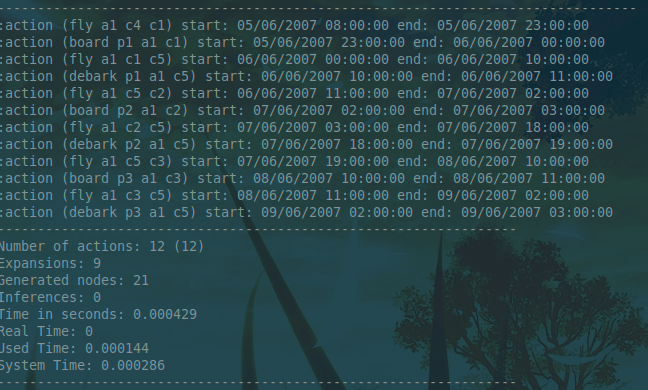
\includegraphics[scale=0.4]{img/e1.png}
\caption{Plan obtenido en el ejercicio 1.}
\end{figure}

\section{Ejercicio 2}

En este ejercicio se ha modificado la tarea de mover el avión para que considere también el repostaje en caso de tener insuficiente
fuel. Si no tiene suficiente, lo único que tiene que hacer primero es repostar y luego volar. A continuación se puede ver
la implementación:

\begin{algorithm}[H]
\begin{lstlisting}[
  caption={Modificación de la tarea de mover avión.},
  label={lst:pddlmove},
  language=PDDL]
(:task mover-avion
 :parameters (?a - aircraft ?c1 - city ?c2 -city)
  
  (:method RefuelFlyAircraft
    :precondition (not (hay-fuel ?a ?c1 ?c2))
    :tasks(
      (refuel ?a ?c1)
      (fly ?a ?c1 ?c2)
    )
  )
)
\end{lstlisting}
\end{algorithm}

También se ha añadido un predicado derivado para comprobar si se tiene suficiente combustible, el cuál es utilizado en la tarea del
movimiento (es el predicado \textbf{hay-fuel}, el cuál está asociado a un avión y mira si hay combustible para ir de \textit{c1} a
\textbf{c2}. El plan que se obtiene del problema se puede ver a continuación:

\begin{figure}[H]
\centering
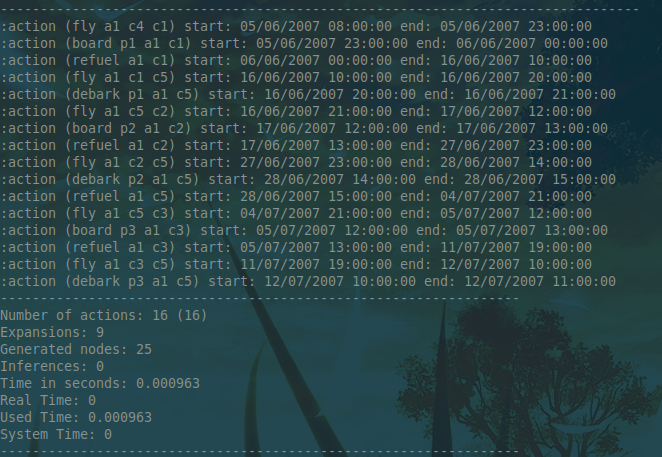
\includegraphics[scale=0.4]{img/e2.png}
\caption{Plan obtenido en el ejercicio 2.}
\end{figure}

\section{Ejercicio 3}

En este ejercicio se ha modificado la tarea de mover el avión para considerar distintos tipos de desplazamientos, priorizando siempre
que se realice lo más rápido posible. Esto se hace al especificar el orden en el que se aplican los métodos. Primero se van a
comprobar aquellos en los que el avión puede realizar un ``\textit{zoom}'', y si no puede, se mirará si puede realizar un vuelo
normal. También se han añadido 2 nuevos predicados derivados para saber si un avión tiene suficiente combustible para hacer un
``\textit{zoom}'' o un vuelo normal, y se ha modificado el predicado derivado del apartado anterior para comprobar si tiene
combustible para los dos tipos de vuelos (cada uno consume una cantidad diferente).

El primer método que se comprueba es si el avión puede realizar un ``\textit{zoom}'' sin repostar, es decir,
si tiene suficiente fuel para ir al destino, y en caso de poder hacerlo, solo se desplazará el avión mediante un ``\textit{zoom}''.
El otro método comprueba si puede desplazarse con un ``\textit{zoom}'' pero sin tener suficiente combustible, en cuyo caso repostará
primero y luego se desplazará mediante un ``\textit{zoom}''. Otro método será si puede realizar un vuelo lento y tiene suficiente
combustible para hacerlo, en cuyo caso volará al destino. Y el último método comprueba si puede realizar un vuelo lento pero no tiene
suficiente combustible, en cuyo caso repostará primero y luego volará.

Debido a que la implementación ocupa demasiadas líneas, la explicación ofrecida anteriormente se considera suficiente y se recomienda
mirar el dominio del ejercicio para ver exactamente como está implementada. Vamos a ver, no obsteante, cuáles son los resultados al
resolver el problema:

\begin{figure}[H]
\centering
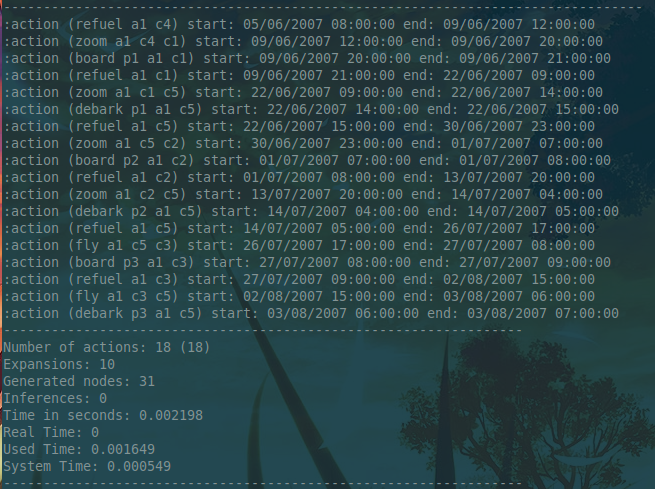
\includegraphics[scale=0.4]{img/e3.png}
\caption{Plan obtenido en el ejercicio 3.}
\end{figure}

\section{Ejercicio 4}

En este ejercicio se han modificado tanto el dominio como las primitivas para poder permitir embarcar múltiples pasajeros, imponer
límites de tiempo para los aviones y cambiar la forma en la que se representa el límite de combustible para hacer que cada avión
tenga el suyo. Con tal de no superar el número máximo de páginas, se van a describir de palabra las modificaciones realizadas, sin
entrar en demasiado detalle en la implementación:

\begin{itemize}[label=\textbullet]
	\item Se han modificado las primitivas \textbf{board} y \textbf{debark}. Ahora la acción de embarcar comprueba que no se haya
	llegado al límite dado de pasajeros para ese avión, y en caso de que no suceda, se embarca el pasajero y se cuenta un nuevo
	pasajero embarcado. En la acción de desembarcar, se comprueba que no se haya vaciado completamente el avión, y en caso de que
	no sea así, se desembarca el pasajero.
	\item Se han creado dos nuevas tareas para embarcar y desembarcar a múltiples pasajeros de forma recursiva, comprobando siempre
	los destinos de las personas para saber si deben o no subir o bajar de ese avión.
	\item Se ha añadido un predicado para representar el destino de una persona determinada, tal y como se ha especificado en el
	enunciado.
	\item Se han añadido una serie de nuevas funciones y predicados derivados. Entre las funcione se incluyen, por ejemplo, el númer
	de pasajeros que lleva un determinado avión en ese momento, la cantidad máxima de pasajeros que puede llevar un avión, el límite
	de tiempo de un avión (un avión no puede realizar un viaje de duración superior al que se le ha especificado en el límite de
	tiempo; si por ejemplo se le ha especificado un límite de tiempo de 20 horas, no puede realizar un vuelo de duración superior)
	y se ha modificado el límite de combustible para que cada avión tenga el suyo propio. En cuanto a los predicados derivados, se han
	añadido dos nuevos predicados que sirven para comprobar si la acción de volar lento o rápido (mediante un ``\textit{zoom}'') se
	pasan del tiempo límite. Estos predicados derivados serán utilizados en las precondiciones de los métodos de vuelo para, además
	de comprobar si se tiene combustible suficiente, comprobar que no se supere el límite de tiempo establecido. Los tiempos se
	calculan utilizando las distancias entre las ciudades y las velocidades.
\end{itemize}

Para especificar las tareas objetivo se tiene que especificar a dónde se quiere transportar cada persona, tal y como se hacía en los
anteriores ejercicios. Por tanto, en las tareas objetivo aparecerán una serie de \textbf{transport-person}, donde la ciudad a la
que se quiere transportar la persona tiene que ser la misma que la ciudad destino.

A continuación se van a explicar brevemente los problemas planteados. Los planes no van a ser incluidos en la memoria, debido
a que son más largos. Si se quieren consultar, se han adjuntado algunos archivos que los contienen.

\subsection{Problema 1}

Se ha planteado un problema con 12 personas y todos los aeropuertos españoles con las mismas distancias que aparecen en el enunciado.
Además, se ha planteado utilizar 6 aviones con velocidades, consumos, capacidades y número máximo de pasajeros distintos. Todos ellos
tienen la misma restricción de tiempo de 300 horas, a las cuáles no van a llegar, siendo por tanto esta restricción inexistente.
El planificador consiguió encontrar un plan, el cuál se puede ver en el archivo \textit{Solucion\_problema1.txt}, donde se puede ver
que alterna entre vuelos rápidos y lentos con cada avión procurando no superar la cantidad máxima de combustible establecido.

\subsection{Problema 2}

Se ha realizado una modificación del problema anterior, cambiando el destino de una persona y reduciendo el número de aviones
a 4. En este caso, el planificador de nuevo consiguió encontrar un plan, alternando los vuelos lentos y las rápidos con tal de
no superar la cantidad máxima de combustible. El resultado se puede ver en \textit{Solucion\_problema2.txt}.

\subsection{Problema 3}

Se ha modificado el problema 1 cambiando las horas máximas de vuelo de cada avión, reduciéndolas, algunas en mayor medida y otras
en menor. El plan obtenido es diferente al que se había obtenido inicialmente, y se puede ver en el archivo \textit{Solucion\_problema3.txt}.

\subsection{Problema 4}

Se ha modificado el problema 1 añadiendo personas hasta un total de 20, modificando los destinos de aquellas personas que ya estaban
en el problema 1. Se han añadido más aviones hasta un total de 9, poniéndoles unas capacidades lo suficientemente grandes para poder
hacer algunos recorridos y modificando el número de horas máximo por trayecto, asignando de forma manual un número de horas razonable,
ya que hay trayectos que llevarían más horas que otros. También se han modificado algunos consumos y velocidades, debido a que en
caso contrario, no se hubiese encontrado una solución satisfactoria al problema. Todas estas decisiones (destinos, consumos,
velocidades, etc.) han sido tomadas a base de probar si el planificador era capaz de encontrar algún plan para una configuración
de predicados y funciones. Debido a que en muchos casos el planificador ha estado hasta un total de 40 minutos sin encontrar ningún
plan, finalmente tras mucho probar se ha escogido la configuración de valores que se ve reflejada en el archivo del problema. Esto
también ha influido en que la mayoría de personas tienen como destino ciudades cercanas a ellos o la misma ciudad en la que están,
ya que cambiando ligeramente la descripción del problema se podía llegar a una en la que no había solución.

Con los valores especificados en la descripción del problema, el planificador pudo encontrar una solución, aunque le llevó algo de
tiempo, más que en los casos anteriores. Esta solución se puede ver en el archivo \textit{Solucion\_problema4.txt}.

\end{document}

